\chapter{РЕЗУЛЬТАТИ ХІРУРГІЧНОГО ЛІКУВАННЯ ПАЦІЄНТІВ З ГЕПАТОБЛАСТОМОЮ}

\section{Порівняльна характеристика оперативних втручань}

Інтраопераційні показники наведено у таблиці (Таб. \ref{tab:operdani})


\begin{table}[]
\centering
\caption{Інтраопераційні показники при резекції і трансплантації печінки.}
\label{tab:operdani}
\begin{tabular}{|p{0.2\linewidth}|
                 p{0.2\linewidth}|
                 p{0.2\linewidth}|
                 p{0.2\linewidth}|}
\hline
{\color[HTML]{231F20} \textbf{Показник}} &
  {\color[HTML]{231F20} \textbf{Резекційна група (n=81)}} &
  {\color[HTML]{231F20} \textbf{Транс\-план\-тацій\-на група (n=9)}} &
  {\color[HTML]{231F20} \textbf{P}} \\ \hline
{\color[HTML]{231F20} \textbf{Час орперації (хв.)}}        & {\color[HTML]{231F20} 240±185} & {\color[HTML]{231F20} 890±181} & {\color[HTML]{231F20} 0,65} \\ \hline
{\color[HTML]{231F20} \textbf{Крововтрата ( мл.)}}         & {\color[HTML]{231F20} 205±160} & {\color[HTML]{231F20} 460±183} & {\color[HTML]{231F20} 0,68} \\ \hline
{\color[HTML]{231F20} \textbf{Чес теплової ішемії (хв.)}}  & {\color[HTML]{231F20} 30±15}   & {\color[HTML]{231F20} −}       & {\color[HTML]{231F20} 0,72} \\ \hline
{\color[HTML]{231F20} \textbf{Час холодової ішемії (хв.)}} & {\color[HTML]{231F20} −}       & {\color[HTML]{231F20} 55±15}   & {\color[HTML]{231F20} 0,76} \\ \hline
{\color[HTML]{231F20} \textbf{Кількість релапаротомій}} &
  {\color[HTML]{231F20} 6 (11,5\%)} &
  {\color[HTML]{231F20} 1 (12,5\%)} &
  {\color[HTML]{231F20} 0,93} \\ \hline
{\color[HTML]{231F20} \textbf{Тривалість п/о періоду}}     & {\color[HTML]{231F20} 21±7}    & {\color[HTML]{231F20} 48±17}   & {\color[HTML]{231F20} 0,63} \\ \hline
{\color[HTML]{231F20} \textbf{Морбідність}}                & {\color[HTML]{231F20} 17,30\%} & {\color[HTML]{231F20} 11,10\%} & {\color[HTML]{231F20} 0,91} \\ \hline
{\color[HTML]{231F20} \textbf{Летальність}}                & {\color[HTML]{231F20} 4 (5\%)} & {\color[HTML]{231F20} 0 (0\%)} & {\color[HTML]{231F20} 0,95} \\ \hline
\end{tabular}
\end{table}

\section{Порівняльна характеристика морфологічних типів  у пацієнтів з гепатобластомою}

(Таб.\ref{tab:patchim})

\begin{table}[]
\centering
\caption{Відповідь пухлини на неоадювантну хіміотерапію в залежності від  гістологічного типу гепатобластоми.}
\label{tab:patchim}
\resizebox{\textwidth}{!}{%
\begin{tabular}{|
>{\columncolor[HTML]{FFFFFF}}l |
>{\columncolor[HTML]{FFFFFF}}l |
>{\columncolor[HTML]{FFFFFF}}l |
>{\columncolor[HTML]{FFFFFF}}l |}
\hline
{\color[HTML]{231F20} \textbf{Тип}} &
  {\color[HTML]{231F20} \textbf{Підтип}} &
  {\color[HTML]{231F20} \textbf{Частота повної або часткової відповіді за RECIST}} &
  {\color[HTML]{231F20} \textbf{Значимість відмінностей, p}} \\ \hline
\cellcolor[HTML]{FFFFFF}{\color[HTML]{231F20} } &
  {\color[HTML]{231F20} \textbf{Фетальний підтип}} &
  {\color[HTML]{231F20} \textbf{26 (96,3\%)}} &
  {\color[HTML]{231F20} \textbf{0,03}} \\ \cline{2-4} 
\cellcolor[HTML]{FFFFFF}{\color[HTML]{231F20} } &
  {\color[HTML]{231F20} Змішаний ембріональний / фетальний підтип} &
  {\color[HTML]{231F20} 15 (93,7\%)} &
  {\color[HTML]{231F20} \textbf{0,04}} \\ \cline{2-4} 
\cellcolor[HTML]{FFFFFF}{\color[HTML]{231F20} } &
  {\color[HTML]{231F20} Макротрабекулярний підтип} &
  {\color[HTML]{231F20} 2 (50,0\%)} &
  {\color[HTML]{231F20} 0,67} \\ \cline{2-4} 
\multirow{-4}{*}{\cellcolor[HTML]{FFFFFF}{\color[HTML]{231F20} \textbf{Епітеліальний тип}}} &
  {\color[HTML]{231F20} Дрібноклітинний недиференційований підтип} &
  {\color[HTML]{231F20} 1 (33,3\%)} &
  {\color[HTML]{231F20} 0,75} \\ \hline
\cellcolor[HTML]{FFFFFF}{\color[HTML]{231F20} } &
  {\color[HTML]{231F20} Без тератоїдних особливостей} &
  {\color[HTML]{231F20} 18 (94,7\%)} &
  {\color[HTML]{231F20} \textbf{0,03}} \\ \cline{2-4} 
\multirow{-2}{*}{\cellcolor[HTML]{FFFFFF}{\color[HTML]{231F20} \textbf{Змішаний тип (епітеліальний та мезенхімальний)}}} &
  {\color[HTML]{231F20} З тератоїдними особливостями} &
  {\color[HTML]{231F20} 17 (94,4\%)} &
  {\color[HTML]{231F20} \textbf{0,04}} \\ \hline
{\color[HTML]{231F20} \textbf{Гепатобластома без додаткових особливостей (NOS)}} &
  {\color[HTML]{231F20} } &
  {\color[HTML]{231F20} 3 (100\%)} &
  {\color[HTML]{231F20} \textbf{0,02}} \\ \hline
\end{tabular}%
}
\end{table}

\section{Загальна характеристика післяопераційного періоду}
Порівняльна характеристика функціонального стану печінки.

Рисунок 5.8 Динаміка загального білка

Рисунок 5.7 Динаміка загального білірубіну

Рисунок 5.9 Динаміка альбуміну

Рисунок 5.10 Динаміка загального білірубіну

Рисунок 5.11 Динаміка АЛТ

Рисунок 5.12 Динаміка АСТ

Рисунок 5.11 Динаміка ГГТП

Рисунок 5.14 Динаміка ЛФ

Рисунок 5.15 Динаміка ЛДГ

\section{Порівняльна оцінка ранніх післяопераційних результатів}

Ранні післяопераційні ускладнення наведено у таблиці (Таб. \ref{tab:uscladn}). 
Післяопераційні ускладнення згідно класифікації Dindo-Clavien по групах наведено у таблиці (Таб. \ref{tab:dindopac}). 


\begin{table}[]
\centering
\caption{Ранні післяопераційні ускладнення.}
\label{tab:uscladn}

\begin{tabular}{{|p{0.2\linewidth}|
                 p{0.2\linewidth}|
                 p{0.2\linewidth}|
                 p{0.2\linewidth}|}}
\hline
{\color[HTML]{231F20} \textbf{Ускладнення}} &
  {\color[HTML]{231F20} \textbf{Резекційна група (n=81)}} &
  {\color[HTML]{231F20} \textbf{Транс\-план\-тацій\-на група (n=9)}} &
  {\color[HTML]{231F20} \textbf{P}} \\ \hline
{\color[HTML]{231F20} \textbf{Гостра перфоративна виражка кишечника}} &
  {\color[HTML]{231F20} \textbf{2 (2,5\%)}} &
  {\color[HTML]{231F20} \textbf{−}} &
  {\color[HTML]{231F20} \textbf{0,64}} \\ \hline
{\color[HTML]{231F20} \textbf{Ексудативний плеврит}}              & {\color[HTML]{231F20} 2 (2,5\%)} & {\color[HTML]{231F20} 1 (11,1\%)} & {\color[HTML]{231F20} 0,62} \\ \hline
{\color[HTML]{231F20} \textbf{Підтікання жовчі}}                  & {\color[HTML]{231F20} 4 (4,9\%)} & {\color[HTML]{231F20} 1 (11,1\%)} & {\color[HTML]{231F20} 0,8}  \\ \hline
{\color[HTML]{231F20} \textbf{Інфекція п/о рани}}                 & {\color[HTML]{231F20} 3 (3,7\%)} & {\color[HTML]{231F20} 1 (11,1\%)} & {\color[HTML]{231F20} 0,64} \\ \hline
{\color[HTML]{231F20} \textbf{Пневмонія}}                         & {\color[HTML]{231F20} 3 (3,7\%)} & {\color[HTML]{231F20} 1 (11,1\%)} & {\color[HTML]{231F20} 0,57} \\ \hline
{\color[HTML]{231F20} \textbf{Сепсис, поліорганна недостатність}} & {\color[HTML]{231F20} 2 (2,5\%)} & {\color[HTML]{231F20} −}          & {\color[HTML]{231F20} 0,57} \\ \hline
{\color[HTML]{231F20} \textbf{Внтурішньо\-очеревна кровотеча}}       & {\color[HTML]{231F20} 2 (2,5\%)} & {\color[HTML]{231F20} −}          & {\color[HTML]{231F20} 0,95} \\ \hline
{\color[HTML]{231F20} \textbf{Шлунково-кишкова кровотеча}}        & {\color[HTML]{231F20} 1 (1,2\%)} & {\color[HTML]{231F20} −}          & {\color[HTML]{231F20} }     \\ \hline
\end{tabular}
\end{table}


\begin{table}[]
\centering
\caption{Післяопераційні ускладнення по класифікації Dindo-Clavien.}
\label{tab:dindopac}

\begin{tabular}{|p{0.2\linewidth}|
                 p{0.2\linewidth}|
                 p{0.2\linewidth}|
                 p{0.2\linewidth}|}
\hline
{\color[HTML]{231F20} \textbf{Cтyпiнь}} &
  {\color[HTML]{231F20} \textbf{Резекційна група (n=81)}} &
  {\color[HTML]{231F20} \textbf{Транс\-план\-тацій\-на група (n=9)}} &
  {\color[HTML]{231F20} \textbf{P}} \\ \hline
{\color[HTML]{231F20} \textbf{I}} &
  {\color[HTML]{231F20} \textbf{4}} &
  {\color[HTML]{231F20} \textbf{1}} &
  {\color[HTML]{231F20} \textbf{0,64}} \\ \hline
{\color[HTML]{231F20} \textbf{II}}   & {\color[HTML]{231F20} 1} & {\color[HTML]{231F20} 1} & {\color[HTML]{231F20} 0,62} \\ \hline
{\color[HTML]{231F20} \textbf{IIIa}} & {\color[HTML]{231F20} 5} & {\color[HTML]{231F20} 1} & {\color[HTML]{231F20} 0,8}  \\ \hline
{\color[HTML]{231F20} \textbf{IIIb}} & {\color[HTML]{231F20} 4} & {\color[HTML]{231F20} 1} & {\color[HTML]{231F20} 0,64} \\ \hline
{\color[HTML]{231F20} \textbf{IVa}}  & {\color[HTML]{231F20} 2} & {\color[HTML]{231F20} −} & {\color[HTML]{231F20} 0,57} \\ \hline
{\color[HTML]{231F20} \textbf{IVb}}  & {\color[HTML]{231F20} 2} & {\color[HTML]{231F20} −} & {\color[HTML]{231F20} 0,57} \\ \hline
{\color[HTML]{231F20} \textbf{V}}    & {\color[HTML]{231F20} 4} & {\color[HTML]{231F20} −} & {\color[HTML]{231F20} 0,95} \\ \hline
\end{tabular}
\end{table}


\section{Порівняльна оцінка віддалених післяопераційних результатів}

Загальна виживаність пацієнтів з гепатобластомою наведена у графіку (Рис. \ref{fig:os})
\begin{figure}[h]
\caption{Загальна виживаність пацієнтів з гепатобластомою.}
\centering
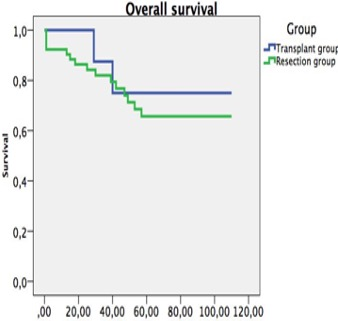
\includegraphics[width=0.6\textwidth]{Illustrations/os.jpg}
\label{fig:os} 
\end{figure}

Безрецидивана виживаність пацієнтів з гепатобластомою наведена у графіку (Рис. \ref{fig:dfs})

\begin{figure}[h]
\caption{Безрецидивана виживаність пацієнтів з гепатобластомою.}
\centering
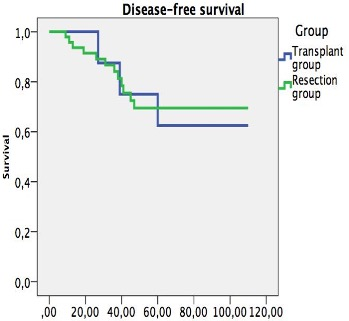
\includegraphics[width=0.6\textwidth]{Illustrations/dfs.jpg}
\label{fig:dfs} 
\end{figure}



\section{Алгоритм вибору тактики лікування у пацієнтів з гепатобластомою}
Нами було розроблено алгоритм вибору тактики лiкування у пацiєнтiв з гепатобластомою (Рис. \ref{fig:algoritm})
\begin{figure}[h]
\caption{Алгоритм діагностики і лікування гепатобластоми в залежності від групи ризику}
\centering
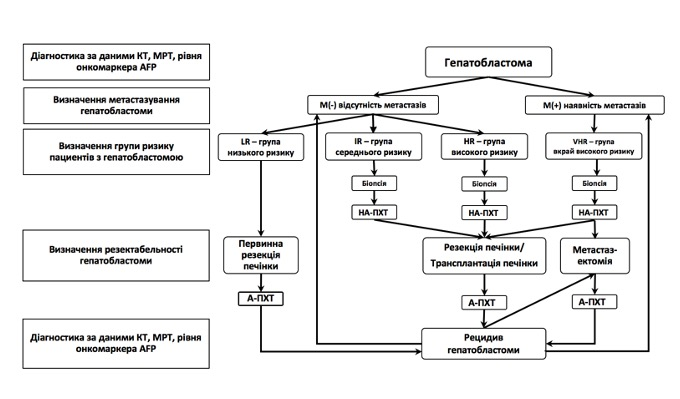
\includegraphics[width=0.9\textwidth]{Illustrations/algoritm.jpg}
\label{fig:algoritm} 
\end{figure}